\documentclass[11pt]{article}
%%%%%%%%%%%%%%%%
% Packages
%%%%%%%%%%%%%%%%

\usepackage[top=1cm,bottom=1cm,left=1.5cm,right= 1.5cm]{geometry}
\usepackage[parfill]{parskip}
\usepackage{graphicx, fontspec, xcolor,multicol, enumerate, setspace}
\DeclareGraphicsRule{.tif}{png}{.png}{`convert #1 `dirname #1`/`basename #1 .tif`.png}

%%%%%%%%%%%%%%%%
% No page number
%%%%%%%%%%%%%%%%

\pagestyle{empty}

%%%%%%%%%%%%%%%%
% User defined colors
%%%%%%%%%%%%%%%%

% Pantone 2015 Spring colors
% http://iwork3.us/2014/09/16/pantone-2015-spring-fashion-report/
% update each semester or year

\xdefinecolor{custom_blue}{rgb}{0, 0.70, 0.79} % scuba blue
\xdefinecolor{custom_darkBlue}{rgb}{0.11, 0.31, 0.54} % classic blue
\xdefinecolor{custom_orange}{rgb}{0.97, 0.57, 0.34} % tangerine
\xdefinecolor{custom_green}{rgb}{0.49, 0.81, 0.71} % lucite green
\xdefinecolor{custom_red}{rgb}{0.58, 0.32, 0.32} % marsala

\xdefinecolor{custom_lightGray}{rgb}{0.78, 0.80, 0.80} % glacier gray
\xdefinecolor{custom_darkGray}{rgb}{0.54, 0.52, 0.53} % titanium

%%%%%%%%%%%%%%%%
% Coloring titles, links, etc.
%%%%%%%%%%%%%%%%

\usepackage{titlesec}
\titleformat{\section}
{\color{custom_blue}\normalfont\Large\bfseries}
{\color{custom_blue}\thesection}{1em}{}
\titleformat{\subsection}
{\color{custom_blue}\normalfont}
{\color{custom_blue}\thesubsection}{1em}{}

\newcommand{\ttl}[1]{ \textsc{{\LARGE \textbf{{\color{custom_blue} #1} } }}}

\newcommand{\tl}[1]{ \textsc{{\large \textbf{{\color{custom_blue} #1} } }}}

\usepackage[colorlinks=false,pdfborder={0 0 0},urlcolor= custom_orange,colorlinks=true,linkcolor= custom_orange, citecolor= custom_orange,backref=true]{hyperref}

%%%%%%%%%%%%%%%%
% Instructions box
%%%%%%%%%%%%%%%%

\newcommand{\inst}[1]{
\colorbox{custom_blue!20!white!50}{\parbox{\textwidth}{
	\vskip10pt
	\leftskip10pt \rightskip10pt
	#1
	\vskip10pt
}}
\vskip10pt
}

%%%%%%%%%%%%%%%%
% Timing
%%%%%%%%%%%%%%%%

% 12-15 minutes

%%%%%%%%%%%%%%%%
% Sakai link for course
%%%%%%%%%%%%%%%%

% UPDATE FOR OWN COURSE
% LINK TO ASSIGNMENTS TOOL IN SAKAI

\newcommand{\Sakai}[1]
{\href{https://sakai.duke.edu/portal/site/ba0d1c18-ba55-473f-9d70-b6a1f9559bbe/page/9870858b-a1a9-481e-8497-8a6ffe9e5be2}{Sakai}}

%%%%%%%%%%%
% App Ex number    %
%%%%%%%%%%%

% DON'T FORGET TO UPDATE

\newcommand{\appno}[1]
{4.2}

%%%%%%%%%%%%%%
% Turn on/off solutions       %
%%%%%%%%%%%%%%

% Off
\newcommand{\soln}[1]{
\vskip5pt
}

%% On
%\newcommand{\soln}[1]{
%\textit{\textcolor{custom_darkGray}{#1}}
%}

%%%%%%%%%%%%%%%%
% Document
%%%%%%%%%%%%%%%%

\begin{document}
\fontspec[Ligatures=TeX]{Helvetica Neue Light}

Dr. \c{C}etinkaya-Rundel \hfill Data Analysis and Statistical Inference \\

\ttl{Application exercise \appno{}: \\
Comparing two means, Part 1}

\inst{Submit your responses on \Sakai{}, under the appropriate assignment. Only one submission per team is required. One team will be randomly selected and their responses will be discussed.}

%%%%%%%%%%%%%%%%%%%%%%%%%%%%%%%%%%%%

Trace metals in drinking water affect the flavor and an unusually high concentration can pose a health hazard. Ten pairs of data were taken measuring zinc concentration in bottom water and surface water at 10 randomly sampled locations. The distributions are shown below. We want to evaluate whether the true average concentration in the bottom water \emph{exceeds} that of surface water? Note that water samples collected at the same location, on the surface and in the bottom, cannot be assumed to be independent of each other.

\begin{center}
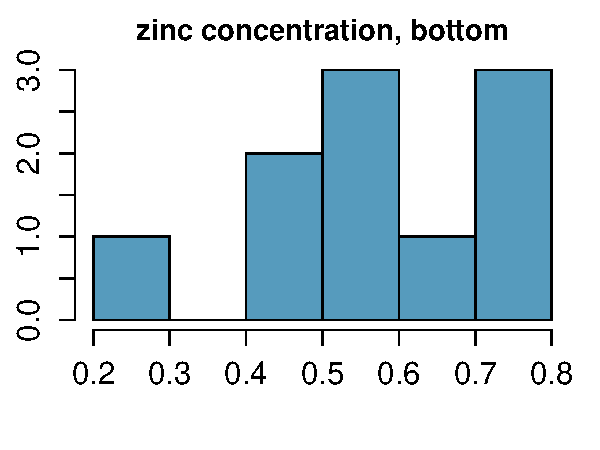
\includegraphics[width=0.35\textwidth]{figures/zinc/zinc_bottom_hist}
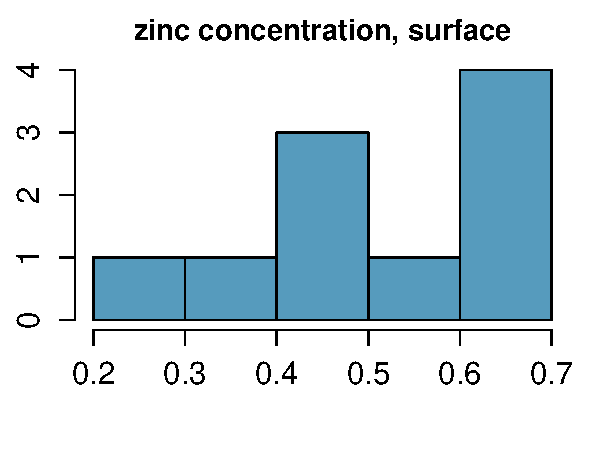
\includegraphics[width=0.35\textwidth]{figures/zinc/zinc_surface_hist}
\end{center}

To complete this application exercise you will need various sample statistics. You can calculate these in R using the raw data. The dataset can be loaded using the following command:
\begin{verbatim}
download("http://stat.duke.edu/~mc301/data/zinc.csv", destfile = "zinc.csv")
zinc = read.csv("zinc.csv")
\end{verbatim}

\begin{enumerate}

\item Define the parameter of interest and the point estimate and calculate the point estimate.

\item Conduct a hypothesis test answering the research question. Don't forget to check conditions first. Use $\alpha = 0.05$. Make sure to frame your conclusion in context of the data and the research question.

\item Calculate a confidence interval for the parameter of interest at the confidence level equivalent to the previous hypothesis test. Make sure to interpret the interval in context of the research question.

\item Describe how you would construct this interval using bootstrapping and the standard error method.

\item Construct the bootstrap interval and compare it to the theoretical interval you calculated earlier.

\end{enumerate}


%\begin{tabular}{c | c | c | c}
%		& bottom	& surface	& difference \\
%\hline
%$\bar{x}$	& 0.5649	& 0.4845	& 0.0804 \\
%$s$		& 0.1468	& 0.1312	& 0.0523 \\
%$n$		& 10		& 10		& 10
%\end{tabular}

%%%%%%%%%%%%%%%%%%%%%%%%%%%%%%%%%%%%
















\end{document}